% title: response.tex
% description: Response to eLife Reviewers
% author: twab

% USAGE: 
% to compile this document:
%    R  >>> knitr::knit("response.Rnw")
%    sh >>> pdflatex response.tex





% latex document setup

\documentclass[11pt]{elife}\usepackage[]{graphicx}\usepackage[]{color}
% maxwidth is the original width if it is less than linewidth
% otherwise use linewidth (to make sure the graphics do not exceed the margin)
\makeatletter
\def\maxwidth{ %
  \ifdim\Gin@nat@width>\linewidth
    \linewidth
  \else
    \Gin@nat@width
  \fi
}
\makeatother

\definecolor{fgcolor}{rgb}{0.345, 0.345, 0.345}
\newcommand{\hlnum}[1]{\textcolor[rgb]{0.686,0.059,0.569}{#1}}%
\newcommand{\hlstr}[1]{\textcolor[rgb]{0.192,0.494,0.8}{#1}}%
\newcommand{\hlcom}[1]{\textcolor[rgb]{0.678,0.584,0.686}{\textit{#1}}}%
\newcommand{\hlopt}[1]{\textcolor[rgb]{0,0,0}{#1}}%
\newcommand{\hlstd}[1]{\textcolor[rgb]{0.345,0.345,0.345}{#1}}%
\newcommand{\hlkwa}[1]{\textcolor[rgb]{0.161,0.373,0.58}{\textbf{#1}}}%
\newcommand{\hlkwb}[1]{\textcolor[rgb]{0.69,0.353,0.396}{#1}}%
\newcommand{\hlkwc}[1]{\textcolor[rgb]{0.333,0.667,0.333}{#1}}%
\newcommand{\hlkwd}[1]{\textcolor[rgb]{0.737,0.353,0.396}{\textbf{#1}}}%
\let\hlipl\hlkwb

\usepackage{framed}
\makeatletter
\newenvironment{kframe}{%
 \def\at@end@of@kframe{}%
 \ifinner\ifhmode%
  \def\at@end@of@kframe{\end{minipage}}%
  \begin{minipage}{\columnwidth}%
 \fi\fi%
 \def\FrameCommand##1{\hskip\@totalleftmargin \hskip-\fboxsep
 \colorbox{shadecolor}{##1}\hskip-\fboxsep
     % There is no \\@totalrightmargin, so:
     \hskip-\linewidth \hskip-\@totalleftmargin \hskip\columnwidth}%
 \MakeFramed {\advance\hsize-\width
   \@totalleftmargin\z@ \linewidth\hsize
   \@setminipage}}%
 {\par\unskip\endMakeFramed%
 \at@end@of@kframe}
\makeatother

\definecolor{shadecolor}{rgb}{.97, .97, .97}
\definecolor{messagecolor}{rgb}{0, 0, 0}
\definecolor{warningcolor}{rgb}{1, 0, 1}
\definecolor{errorcolor}{rgb}{1, 0, 0}
\newenvironment{knitrout}{}{} % an empty environment to be redefined in TeX

\usepackage{alltt}
\usepackage{amsmath}
\usepackage{amssymb}
\usepackage{amsthm}
\usepackage{ragged2e}
\usepackage{caption}
\usepackage{fancyhdr}
\usepackage{graphicx}
\usepackage{titlesec}
\usepackage{blkarray}
\usepackage{csquotes}

% location of figures
\graphicspath{ {./figs/} }


\title{Supplementary Methods\\
\small{Genetic Disruption of WASHC4 Drives Endo-lysosomal Dysfunction and \\
Cognitive-Movement Impairments in Mice and Humans}}


% Authors
\author[1\authfn{0}]{Jamie Courtland}
\author[1\authfn{0}]{Tyler W. A. Bradshaw}
\author[2]{Greg Waitt}
\author[2,3]{Erik J. Soderblom}
\author[2]{Tricia Ho}
\author[4]{Anna Rajab}
\author[5]{Ricardo Vancini}
\author[2\authfn{1}]{Il Hwan Kim}
\author[6]{Ting Huang}
\author[6]{Olga Vitek}
\author[3]{Scott H. Soderling}

\affil[1]{Department of Neurobiology, Duke University School of Medicine, 
Durham, NC 27710, USA}
\affil[2]{Proteomics and Metabolomics Shared Resource, 
Duke University School of Medicine, Durham, NC 27710, USA}
\affil[3]{Department of Cell Biology, Duke University School of Medicine, 
Durham, NC 27710, USA}
\affil[4]{Burjeel Hospital, VPS Healthcare, Muscat, Oman}
\affil[5]{Department of Pathology, Duke University School of Medicine, 
Durham, NC 27710, USA}
\affil[6]{Khoury College of Computer Sciences, Northeaster University,
Boston, MA 02115, USA}

\contrib[\authfn{0}]{These authors contributed equally to this work.}
\presentadd[\authfn{1}]{Department of Anatomy and Neurobiology, 
University of Tennessee Health Science Center, Memphis, TN 38163, USA}

\corr{jlc123@duke.edu}{JC}
\corr{tyler.w.bradshaw@duke.edu}{TWAB}
\corr{greg.waitt@duke.edu}{GW}
\corr{erik.soderblom@duke.edu}{EJB}
\corr{tricia.ho@duke.edu}{TH}
\corr{drannarajab@gmail.com}{DR}
\corr{ricardo.vancini@duke.edu}{RV}
\corr{ikim9@uthsc.edu}{IK}
\corr{huang.tin@northeastern.edu}{TH}
\corr{o.vitek@northeastern.edu}{OV}
\corr{scott.soderling@duke.edu}{SHS}

% reduce space above and below equations
\setlength{\abovedisplayskip}{1pt}
\setlength{\belowdisplayskip}{1pt}


% main
\IfFileExists{upquote.sty}{\usepackage{upquote}}{}
\begin{document}

\maketitle


% abstract
\begin{abstract}

In the review of this manuscript, significant concerns were raised by the
reviewers about the validity of our statistal approach to perform protein- and 
module-level inference from our \textbf{WASH-BioID} and \textbf{SWIP-TMT} 
proteomics datasets. Our previous statistical approach relied upon the R 
package \texttt{edgeR} to evaluate differential protein abundance.
\texttt{edgeR} utilizes a negative binomial, generalized linear
model (NB GLM) framework, fitting each protein with a NB GLM. 
Previously, we failed to fully consider 
the validity of the NB GLM model used by \texttt{edgeR} for proteomics data. 
In response to this critique, we explore the goodness-of-fit of the NB GLM model
for our \texttt{SWIP-TMT} data, and find evidence of a lack-of-fit.
Thus, we revised our statistical approach and reanlyzed our data making use of
the recently published tool \texttt{MSstatsTMT}. \texttt{MSstatsTMT} uses a 
linear mixed model (LMM) framework to model 
major sources of variation in a proteomics experiment. We extend the LMM
framework used by \texttt{MSstatsTMT} to re-evaluate both protein- and 
module-level statistical comparisions. 
Despite evidence of a lack-of-fit for the NB GLM 
method used by \texttt{edgeR}, we find that the inferences we derived from our 
previous analysis are largely preserved in our reanalysis using 
\texttt{MSstatsTMT}.
	
\end{abstract}


\newpage


\section{Lack-of-fit of the Negative Binomial Model}

Our previous approach is summarized as the 'Sum + IRS' method by Huang
\textit{et al.} (REF). Following protein summarization and Internal Reference
Scaling (IRS) normalization, we applied \texttt{edgeR} to assess differential
abundance of individual proteins and protein-groups or modules. 
We drew precidence for the use of \texttt{edgeR} from previous work by Plubell 
and Khan, \textit{et al.} (REFS) who describe IRS normalization and the use of
\texttt{edgeR} for statistical testing in TMT mass spectrometry experiments. 
We failed however, to consider the overall adequacy of the NB GLM model for our
TMT proteomics data.\\

Statisitical inference in \texttt{edgeR} is performed for each gene or protein
using a negative binomial framework in which the data are assumed to be 
adequately described by a NB distribution parameterized by a dispersion 
parameter, $\phi$. Practically, the dispersion parameter accounts for 
mean-variance relationships observed in proteomics and transcriptomics data. 
\texttt{edgeR} employs empirical Bayes methods that allow for the 
estimation of feature-specific (i.e. gene or protein) biological variation, 
even for experiments with small numbers of biological replicates, as is common 
in transcriptomics and proteomics experiments. This empirical Bayes strategy is 
a strength of the \texttt{edgeR} approach as it reduces the uncertainty of the 
estimates and improves testing power.\\

As signal intensity in protein mass spectrometry is fundamentally related to the
number of ions generated from a ioninized, fragmented protein, we incorrectly
infered that TMT mass spectrometry data can be modeled as negative binomial
count data. Based on this assumption, we justified the use of \texttt{edgeR}.
Here we reconsider the overall adequacy of the \texttt{edgeR} NB GLM model for
TMT mass spectrometry data.\\

To evaluate the overall adequacy of the \texttt{edgeR} model, we plot the 
residual protein deviance statistics of all proteins against their theoretical, 
normal quantiles in a quantile-quantile (QQ) plot \textbf{Figure}.
The QQ plot addresses the question of how similar the observed data are to the
theoretical distribution given by NB GLM fit. A linear relationship between the
observed and theoretical values is an indicator of goodness-of-fit.
Deviation from this linear trend is evidence of a lack-of-fit.\\

Following protein summarization and normalization, the data were fit with 
a simple NB GLM of the form \texttt{Abundance $\sim$ Mixture + Condition} using
\texttt{edgeR's} \texttt{glmFit} function which fits a NB GLM model to each
protein or gene (the sub-subplot summaries) in the data. The dispersion
parameter $\phi$ can take several forms, and \texttt{edgeR} supports three 
different dispersion metrics: 'common', 'trended', and 'tagwise'. 
\textbf{Figure} illustrates the divergence of the observed deviance statistics 
from the theoretical distribution for data fit with the NB GLM model. 
These plots emphasize the overall lack of fit of proteomics data 
fit by the \texttt{edgeR} model.\\ 


\section{Reanalysis of SWIP\textsuperscript{P1019R} TMT Proteomics}

Of note, most tools for analysis of protein mass spectromety data are derived
from tools originally developed for analysis of genomics and transcriptomics
data. An exception to this norm is \texttt{MSstatsTMT}, an extension of 
\texttt{MSstats} for analysis of TMT proteomics experiments.\\

\texttt{MSstatsTMT} utilizes a linear mixed-model framework. The strength of
LMMs is their flexibility. LMMs model what we are interested in as a function of
the complex variation in an experimental design. Using LMMs we untagle whate we
are intested in from experimental and biological covariates which mask that
response.  In mixed models, the response variable is taken to be a function of
both fixed and mixed effects.  If the set of possible levels of the covariate is
fixed and reproducible then the factor is modeled as a fixed-effect parameter.
In contrast, if the levels of an observation reflect a random sampling of the
set of all possible levels then the covariate is modeled as a random effect.
Random or mixed-effects represent categorical variables
that reflect experimental or observational "units" in the data set. 
Mixed-effect parameters thus account for the variation occurring among all of the 
lower level units of a particular upper level unit in the data. For this reason,
mixed models may also be refered to as heirarchical models.\\

Tandem mass tag, or TMT reagents enable the combination and simultaneous
quantifiaction of muliple biological samples by mass spectrometry. Currently
commercially available reagents are capable of labeling up to 16 protein
preparations which are then analyzed together in a single mass spectrometry run.
Peptides labeled with TMT tags are distinuisable from each other due to the
unique reporter ions generated by the TMT tag which  is used for relative
quantification.  In a TMT experiment, ionized features are matched to peptides,
these peptide spectrum matches (PSM), for all unique TMT channels are analyzed
simultaneously as a single precursor. Quantification of all biological
conditions is thus achived within a single MS run in which all features for a
protein are quantified simultaneously.\\

Huang \textit{et al.} created \texttt{MSstatsTMT}, an R package for data
normalization and hypothesis testing in multiplex TMT proteomics experiments. 
They outline a common vocabulary for describing the experimental design of 
TMT MS experiments. A TMT experiment consists
of the analysis of \texttt{m = 1} ... \texttt{M}\ concatensions of isobarically
labeled samples or \texttt{Mixtures}. This mixture is then analyzed by the mass
spectrometer in a mass spectrometry \texttt{Run}. This mixture is often
fractionated into multiple liquid chromotography \texttt{Fractions} to decrease
sample complexity, and thereby increase the depth of proteome coverage. 
Within a mixture, each of the unique TMT channels is dedicated to the 
analysis of \texttt{c = 1} ... \texttt{C}\ individual biological or treatment 
\texttt{Conditions}.  There may then be \texttt{b = 1} or more \texttt{B}\ 
biological replicates or \texttt{Subjects}. Finally, a sigle TMT mixture may be 
repeatedly analyzed in \texttt{t = 1} ... \texttt{T}\ technical replicate mass 
spectrometry runs.\\

Protein-wise comparisons between \texttt{Conditions} of \texttt{Subjects} is 
performed by contrast of conditioned means obtained from fitting the data with a
linear mixed-effects model expressing the major sources of variation in the
experimental design. \textbf{Equation} is a mixed-effects model which describes
protein abundance, the response $Y_{mcbt}$, in an experiment composed of
\texttt{M} mixtures, \texttt{T} technical replicates of mixture, \texttt{C}
conditions, and \texttt{B} biological subjects.\\

\begin{equation}
	% full model
	Y_{mcbt} = \mu + Mixture_m + TechRep(Mixture)_{m(t)} + Condition_c + 
	Subject_b + \epsilon_{mcbt}
\end{equation}


\begin{equation}
  \begin{gathered}
	% constraints:
	Mixture_m \stackrel{iid}{\sim} N(0,\sigma^2_M)
	TechRep(Mixture)_{t(m)} \stackrel{iid}{\sim} N(0,\sigma^2_T) \\
	\sum_{c=1}^{C} Condition_c = 0 \\
	Subject_{mcb} \stackrel{iid}{\sim} N(0,\sigma^2_S) \\
	\epsilon{mtcb} \stackrel{iid}{\sim} N(0,\sigma^2) \\
  \end{gathered}
\end{equation}


The model's constraints distinguish fixed and random components of 
variation in the response. \texttt{Mixture} is a mixed effect and 
represents the variation between TMT mixtures which is assumed to be random 
and normally distributed. \texttt{TechRep(Mixture)} represents random variation 
between replicate mass spectrometry runs of a same mixture. 
The term \texttt{Subject} cooresponds to each biological replicate and 
represents biological variation among the levels of the fixed effect term
\texttt{Condition}. The term $\epsilon_{mtcb}$,
is a random-effect representing both biological and technical variation, 
quantifying any remaining error, assumed to be be independent 
and identically distributed.\\

If a component of the model is not estimable, it is removed. 
For example, if there is
no technical replication of mixture (T=0), the model is reduced to: \\

\begin{equation} 
	% reduced model (fx0)
	Y_{mcbt} = \mu + Mixture_m + Condition_c + \epsilon_{mcb}
\end{equation}

In the reduced model, biological variation among individual subjects is 
captured by the term \texttt{Condition} and is thus ommited.\\


\section{Test Statistic}

Model based testing of differential abundance between pairs of conditions
is obtained by comparing the estimates of coefficients of interest. 
We are interested in tested the null hypothesis of 
equality of conditioned means $H0 : l^T\beta = 0$ (lmerTest, Kutzenova2017).
Kutzenova et al derive a test statistic for such contrasts as:\\

\begin{equation}
	% t-statistic
	t = \frac{l^T \hat{\beta}}{\sqrt{l \sigma^2 \hat{V} l^T}}
\end{equation}

We obtain the model estimates $\hat{\beta}$, 
error $\sigma^2$, and
variance-covariance matrix $\hat{V}$ from the fitted model. 
Together $\sigma^2 * \hat{V}$ is the scaled variance-covariance matrix
describing the error estimates of the models mixed-effect parameters. 
Given $l^T$, a vector of sum 1 specifying the positive and negative
coefficients of the comparison, the numerator of the equation is then
the fold change of a given comparison, and together the denominator 
represents the standard error of the contrast. \\

The degrees of freedom for the contrast are derived using the Satterthwaite
moment of approximation method as previously described by Kutzenova et al.
Finally, given the t-statistic, which is assumed to follow an approximate
$chi^2$ distribution, and the degrees of freedom, a p-value is calculated for
the test statistic.  P-values for the protein-wise tests are adjusted using the
Benjamnii hochberg method.\\


\section{SWIP-TMT Proteomics Experimental Design}

We prepared 7 \texttt{BioFractions} from 'Control' and 
SWIP\textsuperscript{P1019R} 'Mutant' mice. Thus in our experiment, 
the fixed effect term \texttt{Condition} of Equation 1 represents the interaction 
of \texttt{Genotype} and \texttt{BioFraction} and is the 14 unique combinations 
of 7 subcellular \texttt{BioFractions} prepared from 'Control' and 'Mutant' mice. 
Our TMT proteomics experimental design is
summarized in \textbf{Figure}.\\

Note that in our experiment each TMT mixture contains seven repeated measurments
made from each biological \texttt{Subject}. We refer to the subcellular
fractions obtained by differential centrifugation of the brain as
\texttt{BioFractions} to distinguish them from MS \texttt{Fractions} in the
\texttt{MSstatsTMT} nomenclator. To account for this source of
intra-Subject variability, we should include the random-effect term
\texttt{Subject} representing the random error within a subject. However, in our
design \texttt{Mixture} is confounded with the term \texttt{Subject} -- in
each mixture we analyzed all \texttt{BioFractions} from a single Control and
Mutant mouse.  Thus we can choose to account for the effect of \texttt{Mixture}
or \texttt{Subject}, but not both. Under the assumption that the effect of TMT
\texttt{Mixture} is greater than the variance attributable to the repeated
measurements of each subject, we omit the term \texttt{Subject}.  The reduced
model is equivalent  to equation (EQ) when condition is
\texttt{Genotype:BioFraction}.\\

\textbf{Figure} shows
the proportion of variance attributable to major covariates in our TMT
experiment for each protein. \\
Given the LMM describing protein abundance as a respones of the experiments
major sources of variaiton, we assessed two different types of contrasts:\\

\begin{enumerate}
	\item 'intra-BioFraction' comparisons for the difference between
		Mutant and Control conditions within a biological fraction.
	\item 'Mutant-Control' contrast for the overall difference between
		Mutant and Control conditions.
\end{enumerate}

The vector $l^T$ is a contrast vector specifying each comparison between the
negative coefficient, e.g. 'GenotypeControl.BioFractionF4' and positive
coefficient, e.g. 'GenotypeMutant.BioFractionF4'. Figure (FIG) shows these two
types of contrast. Contrasts 1-7 specify 'intra-BioFraction' comparisons for
each of the subcellular fractions. Contrast 8 specifies the overall
'Mutant-Control' comparison.\\

\section{Protein-level comparisons}

\texttt{MSstatsTMT} attempts to automatically parse the experimental design and
fit an appropriate LMM for the experimental design. 
In order to understand and extend the function of \texttt{MSstatsTMT}, we 
We extracted \texttt{MSstatsTMT's} core model-fitting and statistical testing 
steps and illustrate them here.\\

%Following data preprocessing, summarization, and normalization, statistical
%inference can be summarized in two steps:\\
%\begin{itemize}
%	\item Fit each protein with the appropriate linear mixed-effects model
%	\item Given the fitted model, assess a contrast of interest 
%\end{itemize}
%		
%At the core of the model fitting step is the
%R package \texttt{lme4} which implements mixed-effects models with its function
%\texttt{lmer}. The package \texttt{lmerTest} extends \texttt{lme4's}
%functionality and enables the computation of the degrees of freedom via the
%Sattertwaite method.\\
%
%%%%%%%%%%%%%%%%%%%%%%%%%%%%%%%%%%%%%%%%%%%%%%%%%%%%%%%%%%%%%%%%%%%%%%%%%%%%%%%%%%
%<<fit0, eval=TRUE, echo=TRUE>>=
%
%library(lmerTest)
%
%library(dplyr)
%library(data.table)
%
%
%# load SwipProteomics data
%data(swip)
%data(msstats_prot)
%
%## the LMM formula to be fit:
%fx0 <- formula("Abundance ~ 0 + Genotype:BioFraction + (1|Mixture)")
%
%# fit the model for WASHC4
%fm0 <- lmer(fx0, msstats_prot %>% filter(Protein == swip))
%
%model_summary <- summary(fm0, ddf = "Satterthwaite")
%
%model_summary$coefficients %>% knitr::kable()
%
%@
%
%%%%%%%%%%%%%%%%%%%%%%%%%%%%%%%%%%%%%%%%%%%%%%%%%%%%%%%%%%%%%%%%%%%%%%%%%%%%%%%%%%
%
%%The model's estimates, $\beta$, represent our best estimate of the mean protein
%%abundance in the 14 conditions of Genotype:BioFraction. We define a contrast
%%to compare the coefficients 'GenotypeMutant:BioFractionF7' and
%%'GenotypeControl:BioFractionF7' to assess the intra-BioFraction
%%difference between Control and Mutant for F4. The model-based comparisons
%%for a given contrast is implemented by our function \texttt{lmerTestContrast}. 
%%This function takes as input a model fitted by
%%\texttt{lmerTest::lmer} and a contrast vector specifying the
%%comparison of interest.\\
%%
%%%%%%%%%%%%%%%%%%%%%%%%%%%%%%%%%%%%%%%%%%%%%%%%%%%%%%%%%%%%%%%%%%%%%%%%%%%%%%%%%
%%%<<contrast0, eval=TRUE, echo=TRUE>>=
%%%
%%%# create a contrast
%%%coeff <- lme4::fixef(fm0)
%%%contrast0 <- setNames(rep(0,length(coeff)), nm = names(coeff))
%%%contrast0["GenotypeMutant:BioFractionF7"] <- +1 # positive coeff
%%%contrast0["GenotypeControl:BioFractionF7"] <- -1 # negative coeff
%%%
%%%# evaluate contrast
%%%lmerTestContrast(fm0,contrast0) %>% knitr::kable()
%%%
%%%@
%%%%%%%%%%%%%%%%%%%%%%%%%%%%%%%%%%%%%%%%%%%%%%%%%%%%%%%%%%%%%%%%%%%%%%%%%%%%%%%%%
%%
%%It is useful to consider the goodness-of-fit of our model. Here we  
%%assess the goodness-of-fit of each protein-wise LMM using Nagagawa's
%%coefficient of determination, as implemented by the 
%%\texttt{r.squaredGLMM.merMod} function forked from the \texttt{MuMin} package.\\
%%A goodness-of-fit metric is the coefficient of determination.
%%Nakagawa describes a generalized description of the coefficient of determination
%%for LMM. R2c, for conditional effects, quantifies the total variation explained 
%%by the model. R2m, for marginal, quantifies the variation explained by fixed effects.
%%We refer to R2 conditional here as $R^2_{total}$ as it quantifies the total
%%variance explained by the LMM. $R^2_{fixed}$ is the variation
%%explained by the models marginal parameters.
%%
%%We can see the total variation explained by the model is 0.949. The variance
%%explained by fixed effects Genotype and BioFraction equates to 0.935. Thus
%%approximately 1.5\% of the remaing variance is attributable to mixed effects and
%%residual variance.
%%
%%%%|Protein |Symbol | Entrez|  R2.fixef|  R2.total|
%%%%|:-------|:------|------:|---------:|---------:|
%%%%|Q3UMB9  |Washc4 | 319277| 0.9353344| 0.9494330|
%%
%%
%%%%%%%%%%%%%%%%%%%%%%%%%%%%%%%%%%%%%%%%%%%%%%%%%%%%%%%%%%%%%%%%%%%%%%%%%%%%%%%%%
%%%<<<contrast1, eval = TRUE, echo = TRUE >>=
%%%
%%%# use convenience function to contruct a contrast
%%%l1 <- getContrast(fm0, "Mutant","Control")
%%%
%%%results <- lmerTestContrast(fm0, l1)
%%%
%%%results %>% mutate(Contrast - 'Mutant-Control') %>% 
%%%	unique() %>% knitr::kable()
%%%
%%%@
%%%%%%%%%%%%%%%%%%%%%%%%%%%%%%%%%%%%%%%%%%%%%%%%%%%%%%%%%%%%%%%%%%%%%%%%%%%%%%%%%
%%
%%
%%\section{Module-level analysis}
%%
%%We wish to perform inference at the level of protein modules. These groups of
%%covarying proteins represent hypothesized biological niches
%%defined by proteins that localized together in subcellular
%%space.\\
%%
%%Effects are fixed if they are interesting in themselves or random if there is
%%interest in the underlying population. Searle, Casella, and McCulloch (1992,
%%Section 1.4) explore this distinction in depth. morover as the sample does not
%%We are interested in the overall affect on the group of proteins and not the
%%Mixed effects represent a subset of the exhaust the population. A strenght of
%%the LMM approach applied to is the partial pooling which strengthens the power
%%of the statistical test.  Here we hypothesize that covarying protein represetnt
%%groups of proteins that are a part of a larger groups with a common mean effect.
%%Proteins within a module represnt correlated observations with we model as a
%%mixed effect. We take the stance that Protein is a random effect in that we are
%%primarily interested in makein inference about the overall distribution
%%responses for a module rather than within between the particular sublevels of a
%%module.\\
%%
%%We model protein groups or modules by adding the mixed effect term
%%\texttt{Protein}. The protein constituents of a module.\\
%%
%%\begin{equation} 
%%	% module-model (fx1)
%%	Y_{mcbt} = \mu + Mixture_m + Condition_c + Protein_p + \epsilon_{mcb}
%%\end{equation}
%%
%%\begin{equation}
%%  \begin{gathered}
%%	  % constraints:
%%	Protein{p} \stackrel{iid}{\sim} N(0,\sigma^2_P) \\
%%  \end{gathered}
%%\end{equation}
%%
%%%%%%%%%%%%%%%%%%%%%%%%%%%%%%%%%%%%%%%%%%%%%%%%%%%%%%%%%%%%%%%%%%%%%%%%%%%%%%%%%%
%%%<<<>>=
%%%## the module-level model to be fit:
%%%washc_prots = mapID("Washc*")
%%%form <- "Abundance ~ (1|Genotype) + (1|BioFraction) + (1|Mixture) + (1|Protein)"
%%%
%%%# warnings because our module is too perfect
%%%fit <- suppressWarnings({ lmerTest::lmer(form, msstats_prot %>% filter(Protein %in% washc_prots)) })
%%%
%%%# calculate partitioned variance
%%%mixef_var <- as.data.frame(lme4::VarCorr(fit,comp="Variance"))
%%%x <- setNames(mixef_var$vcov,nm=mixef_var$grp) # variance of each component
%%%PVE_washc = x/sum(x)
%%%PVE_washc %>% knitr::kable()
%%%@
%%%%%%%%%%%%%%%%%%%%%%%%%%%%%%%%%%%%%%%%%%%%%%%%%%%%%%%%%%%%%%%%%%%%%%%%%%%%%%%%%
%%
%%Again, we consider the variance explained by the model as a measure of its
%%overall quality. Nakagawa's coefficient of determination does not consider the
%%variance explained by mixed affects alone.  The R package
%%\texttt{VariancePartition} computes the varation explained by a LMM terms.
%%percent variance attributable to that term for the mixed-effect model fit to
%%each module.  For each model fit the module-level data, we asses the proprotion
%%of variance explained by \texttt{BioFraction}, \texttt{Genotype},
%%\texttt{Mixture}, and \texttt{Protein}, and \texttt{Residual} variance.
%%
%%%%%%%%%%%%%%%%%%%%%%%%%%%%%%%%%%%%%%%%%%%%%%%%%%%%%%%%%%%%%%%%%%%%%%%%%%%%%%%%%%
%%%<<<>>=
%%%# calculate partitioned variance
%%%mixef_var <- as.data.frame(lme4::VarCorr(fit,comp="Variance"))
%%%x <- setNames(mixef_var$vcov,nm=mixef_var$grp) # variance of each component
%%%PVE_washc = x/sum(x)
%%%PVE_washc %>% knitr::kable()
%%%@
%%%%%%%%%%%%%%%%%%%%%%%%%%%%%%%%%%%%%%%%%%%%%%%%%%%%%%%%%%%%%%%%%%%%%%%%%%%%%%%%%
%%
%%
%%
%%%%%%%%%%%%%%%%%%%%%%%%%%%%%%%%%%%%%%%%%%%%%%%%%%%%%%%%%%%%%%%%%%%%%%%%%%%%%%%%%
%%
%%%% figure 1 -- nb glm and lmm GOF
%%
%%\begin{figure}[ht]
%%	\begin{fullwidth}
%%		\begin{center}
%%		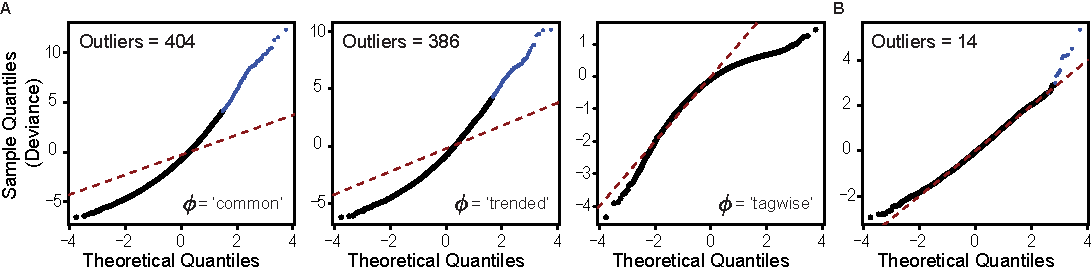
\includegraphics[width=0.9\paperwidth,keepaspectratio]{gof}
%%		\caption{\textbf{Goodness-of-fit of \texttt{edgeR} (A), and 
%%		\texttt{MSstatsTMT} (B) statistical approaches.} The overall
%%		adequacy of the linear models fit to the data were assessed 
%%		by plotting the residual deviance for all proteins as a 
%%		quantile-quantile plot (McCarthy \textit{et al.}, (2012)). 
%%		\textbf{(A)} For analysis with \texttt{edgeR}, The normalized
%%		protein data from \texttt{MSstatsTMT} were fit with a negative
%%		binomal generalized linear model (NBGLM) of the form: 
%%		\texttt{Abundance} $\sim$ \texttt{Mixture + Condition}.
%%		Where \texttt{Mixure} is an additive blocking factor that 
%%		accounts for variablity between experiments. 
%%		The NB framework used by edgeR utilizes a dispersion parameter 
%%		to account for mean-variance relationships in the data.
%%		The dispersion parameter can take several forms. 
%%                \texttt{edgeR} supports three dispersion models: 'common',
%%		'trended', and 'tagwise'. However, when using \texttt{edgeR's}
%%		robust quasi-likelihood test methods, only global (i.e. 'common'
%%		or 'trended') dispersion metrics are appropriate 
%%		(see \texttt{edgeR::glmQLFit's} documentation). 
%%		We plot the protein-wise deviance from the data fit withe ach of
%%		the disperions parameters. Protein-wise deviance
%%		statistics were transformed to normality and plotted against
%%		theoretical normal quantiles using the \texttt{edgeR::gof}
%%		function. \textbf{(B)} For analysis with \texttt{MSstatsTMT},
%%		the normalized protein data were fit with a linear mixed-effects 
%%		model (LMM) of the form: 
%%		\texttt{Abundance} $\sim$ \texttt{0 + Condition + (1|Mixture)}. 
%%		Where \texttt{Mixture} represents the random effect
%%		of \texttt{Mixture}. The residual deviance and degrees of 
%%		freedom were extracted from the fitted models, z-score
%%		normalized, and plotted as in (A). Proteins with a significantly 
%%		poor fit are indicated as outliers in blue 
%%		(Holm-adjusted P-value $<$ 0.05).}
%%		\label{fig:gof}
%%	\end{center}
%%	\end{fullwidth}
%%\end{figure}
%%
%%
%%%% figure 2 -- Experimental Design
%%
%%\begin{figure}[h]
%%  \begin{fullwidth}
%%  \begin{center}
%%	  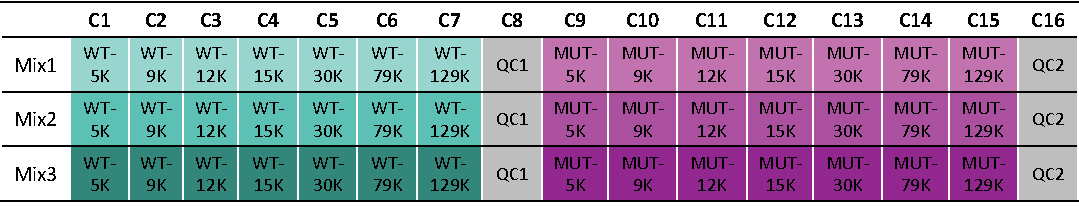
\includegraphics[width=0.9\paperwidth,keepaspectratio]{design}
%%	  \caption{\textbf{Experimental Design.} We performed three 16-plex TMT
%%	  experiments. Each TMT mixture is a concatenation of 16 labeled
%%	  samples. In each experiment we analyzed 7 subcellular
%%	  \texttt{BioFractions} prepared from the brain of a 'Control' or
%%	  'Mutant' mouse. In all we analyzed 3 \texttt{Subjects} from each 
%%	  {Condition}. Each \texttt{Mixture} includes two \texttt{Channels}
%%	  dedicated to the analysis of a common quality control sample.}
%%	  \label{fig:design}
%%  \end{center}
%%  \end{fullwidth}
%%\end{figure}
%%
%%
%%%% figure 3 -- Contrasts
%%
%%\begin{figure}[h]
%%  \begin{fullwidth}
%%  \begin{center}
%%	  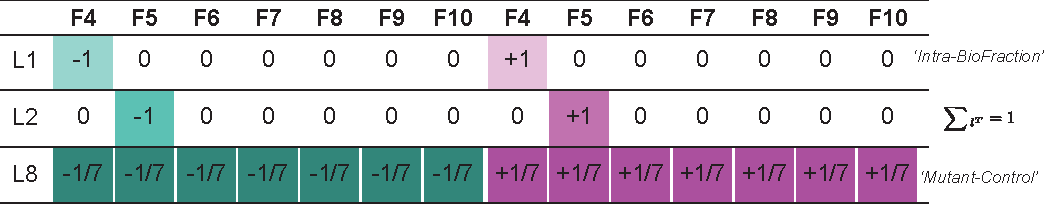
\includegraphics[width=0.9\paperwidth,keepaspectratio]{contrasts}
%%	  \caption{\textbf{Statistical Comparisons.} We assessed two types of
%%	  contrasts. Each row of the matrix specifies a contrast between
%%	  positive and negative coefficients in the mixed effects model fit to
%%	  each protein. Contrasts1-7 are 'intra-BioFraction' contrasts that
%%	  specify the pairwise comparisons of Control and Mutant groups for a
%%	  single fraction. In Contrast 8 we compare 'Mutant-Control' and asses
%%	  the overall difference of 'Control' and 'Mutant' conditions.  Each
%%	  contrast is a vector of sum 1.}
%%	  \label{fig:contrasts}
%%  \end{center}
%%  \end{fullwidth}
%%\end{figure}
%%
%%%% figure 4 -- Variance Partition
%%
%%\begin{figure}[h]
%%  \begin{fullwidth}
%%  \begin{center}
%%	  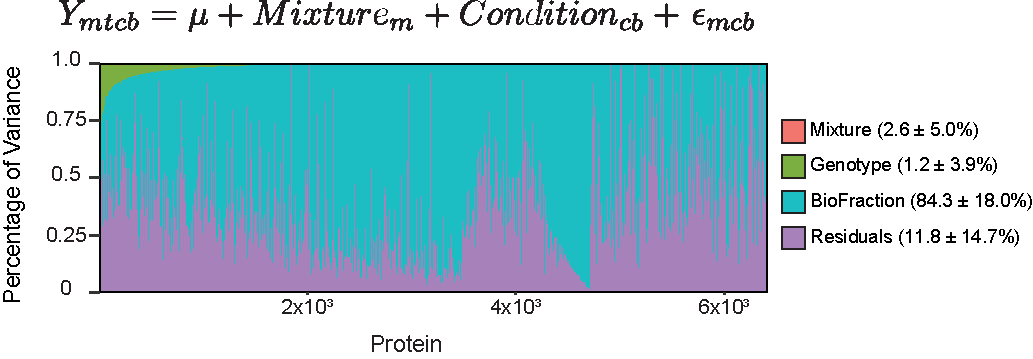
\includegraphics[width=0.9\paperwidth,keepaspectratio]{variance}
%%	  \caption{\textbf{Analysis of Variance Components.} 
%%	  The proportion of variance explained by Genotype, BioFraction,
%%	  Mixture, and remaining residual error (subplot error) for all
%%	  proteins. Note while the contribution of Mixture seems negligiable,
%%	  its average for all proteins is approximately twice the average
%%	  percent variance explained by Genotype. BioFraction explains the
%%	  majority of the variance for all proteins. Analysis done with
%%	  \texttt{variancePartition::calcVarPart}.
%%	  \label{fig:variance}
%%  \end{center}
%%  \end{fullwidth}
%%\end{figure}


\end{document}
